\documentclass[10pt,twocolumn]{article}
\usepackage[margin=0.7in]{geometry}
\usepackage{amsmath,amssymb}
\usepackage{graphicx}
\usepackage{xcolor}
\usepackage{hyperref}
\usepackage{booktabs}
\usepackage{tikz}
\usepackage{titlesec}
\usepackage{enumitem}

\usetikzlibrary{shapes.geometric, arrows, positioning}

% Tighter formatting
\titleformat{\section}{\normalfont\large\bfseries\centering}{\Roman{section}.}{0.5em}{}
\titleformat{\subsection}{\normalfont\normalsize\itshape}{\Alph{subsection}.}{0.5em}{}
\setlist{nosep,leftmargin=*}
\setlength{\parskip}{0.3em}

% TikZ styles
\tikzstyle{block} = [rectangle, rounded corners, minimum width=1.8cm, minimum height=0.5cm, text centered, draw=black, fill=blue!12, font=\footnotesize]
\tikzstyle{arrow} = [thick,->,>=stealth]

\title{\Large\bfseries Analyzing Spotify Audio Features and Discovering Natural Song Clusters }

\author{Sarbani Adhikari\\
\small CS 4412: Data Mining\\
\small Kennesaw State University --- sadhika7@students.kennesaw.edu}

\date{}

\begin{document}

\maketitle

\section{Introduction}

The project seeks to apply data mining techniques to the Spotify Tracks dataset on Kaggle. The purpose of this is to discover natural clusters of songs based on the features provided. Ultimately, we will want to examine each cluster to see if they align or diverge from spotify's existing genre labels and in the process, uncover patterns that may cross traditional genre boundaries.

\section{Dataset Description}

\subsection{Overview}
The Kaggle dataset called Spotify Tracks Dataset provides us with audio features for songs across 125 genres, sourced from the Spotify Web API.

\begin{itemize}
    \item \textbf{Source:} \url{https://www.kaggle.com/datasets/maharshipandya/-spotify-tracks-dataset}
    \item \textbf{Size:} 114,000 rows $\times$ 20 columns (~15 MB)
    \item \textbf{Unique Artists:} 30,119
    \item \textbf{Unique Genres:} 125
\end{itemize}

\subsection{Key Features}
Table~\ref{tab:features} showcases the audio features used for clustering, calculated through Spotify's audio analysis algorithms.

\begin{table}[htbp]
\caption{Audio Features for Clustering}
\label{tab:features}
\centering
\footnotesize
\begin{tabular}{@{}lll@{}}
\toprule
\textbf{Feature} & \textbf{Range} & \textbf{Description} \\
\midrule
danceability & 0.0--1.0 & Suitability for dancing \\
energy & 0.0--1.0 & Intensity and activity \\
valence & 0.0--1.0 & Musical positiveness \\
acousticness & 0.0--1.0 & Acoustic sound confidence \\
instrumentalness & 0.0--1.0 & Absence of vocals \\
speechiness & 0.0--1.0 & Spoken word presence \\
liveness & 0.0--1.0 & Audience presence \\
loudness & dB & Overall loudness \\
tempo & BPM & Beats per minute \\
\bottomrule
\end{tabular}
\end{table}

Additional columns include \texttt{track\_id}, \texttt{artists}, \texttt{album\_name}, \texttt{track\_name}, \texttt{popularity}, \texttt{duration\_ms}, \texttt{key}, \texttt{mode}, and \texttt{track\_genre}.

\subsection{Considerations for Data Quality}
Issues which we may come across while preprocessing:
\begin{itemize}
    \item There may be highly correlated features which can affect clustering 
    \item Tracks could be duplicated or exist across multiple genres 
    \item Labels assigned by Spotify for genre could be inconsistent
    \item The uniqueness of the features means they use different scales
\end{itemize}

\section{Discovery Questions}

\subsection{Primary Question}
\textbf{What natural clusters of songs emerge from audio features, and how do these clusters align or conflict with Spotify's genre labels?}

Although genre classifications can be subjective, audio-based clustering may reveal more information. For example, rock and metal could cluster together while pop may split depending on the energy levels. 

\subsection{Supporting Question 1}
\textbf{What latent dimensions underlie the audio feature space?}

Utilizing PCA, our goal is to reduce features to principal components. From there, we can possibly find interpretable dimensions (such as a mood dimension).

\subsection{Supporting Question 2}
\textbf{What decision rules characterize each cluster's audio profile?}

To generate interpretable rules for the clusters, we'll use decision trees. That would mean having rules that can determine if we have a high energy dance cluster by looking at energy and tempo.

\section{Planned Techniques}

\subsection{Dimensionality Reduction: PCA}
Principal Component Analysis will reduce the feature space for visualization, address multicollinearity, and identify latent dimensions.

\subsection{Clustering: K-Means and DBSCAN}
\textbf{K-Means:} Finds compact clusters; optimal $k$ via Elbow Method and Silhouette Score.

\textbf{DBSCAN:} Density-based; finds arbitrary cluster shapes and identifies outliers.

\subsection{Classification: Decision Trees}
Using each cluster's discovered characteristics, the decision tree can be trained and produce interpretable rules.

\subsection{Validation Metrics}
Silhouette Score, Davies-Bouldin Index, and genre purity/dispersion analysis.

\subsection{Analysis Pipeline}

\begin{figure}[htbp]
\centering
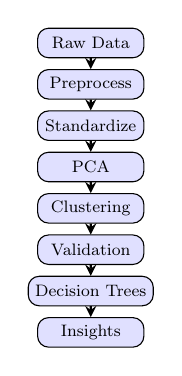
\begin{tikzpicture}[node distance=0.7cm, scale=0.75, transform shape]
    \node (start) [block] {Raw Data};
    \node (prep) [block, below of=start] {Preprocess};
    \node (scale) [block, below of=prep] {Standardize};
    \node (pca) [block, below of=scale] {PCA};
    \node (cluster) [block, below of=pca] {Clustering};
    \node (valid) [block, below of=cluster] {Validation};
    \node (tree) [block, below of=valid] {Decision Trees};
    \node (end) [block, below of=tree] {Insights};
    
    \draw [arrow] (start) -- (prep);
    \draw [arrow] (prep) -- (scale);
    \draw [arrow] (scale) -- (pca);
    \draw [arrow] (pca) -- (cluster);
    \draw [arrow] (cluster) -- (valid);
    \draw [arrow] (valid) -- (tree);
    \draw [arrow] (tree) -- (end);
\end{tikzpicture}
\caption{Analysis Pipeline}
\label{fig:pipeline}
\end{figure}

\section{Preliminary Timeline}

\begin{table}[htbp]
\caption{Project Timeline}
\label{tab:timeline}
\centering
\footnotesize
\begin{tabular}{@{}llp{3.5cm}@{}}
\toprule
\textbf{Milestone} & \textbf{Date} & \textbf{Deliverables} \\
\midrule
M1 & 2/5/26 & Proposal, GitHub setup \\
M2 & 3/10/26 & Preprocessing, EDA, PCA \\
M3 & 4/1/26 & Clustering, validation \\
M4 & 5/1/26 & Decision trees, final report \\
\bottomrule
\end{tabular}
\end{table}

\subsection{Anticipated Challenges}
\begin{enumerate}
    \item \textbf{Feature Scaling:} Different units (BPM vs 0--1) require standardization before clustering.
    \item \textbf{Optimal $k$:} Elbow method may be ambiguous; will compare multiple $k$ values using Silhouette Scores.
    \item \textbf{Genre Granularity:} 125 genres may require grouping for meaningful cluster-genre comparison.
\end{enumerate}

\section{GitHub Repository}

\begin{itemize}
    \item \textbf{Name:} \texttt{cs4412-project-sarbani}
    \item \textbf{URL:} https://github.com/sarbaniadhikari/cs4412-project-sarbani
    \item \textbf{Structure:} \texttt{README.md} (project overview, dataset link), \texttt{data/} (with .gitignore), \texttt{docs/} (proposal), \texttt{notebooks/} (analysis)
\end{itemize}

\begin{thebibliography}{00}
\bibitem{b1} M. Pandya, ``Spotify Tracks Dataset,'' Kaggle, 2022. Available: \url{https://www.kaggle.com/datasets/maharshipandya/-spotify-tracks-dataset}
\end{thebibliography}

\end{document}
